 % cd ..\..\Users\NikitaSkybytskyi\Desktop\c3s1\complex-analysis
\documentclass[a4paper, 12pt]{article}
\usepackage[utf8]{inputenc}
\usepackage[english, ukrainian]{babel}

\usepackage{amsmath, amssymb}
\usepackage{multicol}
\usepackage{graphicx}
\usepackage{float}
\usepackage{multicol}

\usepackage{amsthm}
\newtheorem{theorem}{Теорема}[subsection]
\newtheorem*{theorem*}{Теорема}
\newtheorem{lemma}{Лема}[subsection]
\newtheorem*{lemma*}{Лема}
\newtheorem*{remark*}{Зауваження}
\theoremstyle{definition}
\newtheorem*{definition}{Визначення}
\newtheorem{problem}{Задача}[section]
\newtheorem*{solution}{Розв'язок}
\newtheorem{example}{Приклад}
\newtheorem*{example*}{Приклад}
\newtheorem*{hint}{Вказівка}

\newcommand{\Max}{\displaystyle\max\limits}
\newcommand{\Sum}{\displaystyle\sum\limits}
\newcommand{\Int}{\displaystyle\int\limits}
\newcommand{\Lim}{\displaystyle\lim\limits}

\newcommand{\RR}{\mathbb{R}}
\newcommand{\ZZ}{\mathbb{Z}}

\newcommand*\diff{\mathop{}\!\mathrm{d}}
\newcommand*\Diff[1]{\mathop{}\!\mathrm{d^#1}}

\DeclareMathOperator{\Real}{Re}
\DeclareMathOperator{\Imag}{Im}

\DeclareMathOperator{\Arg}{Arg}

\DeclareMathOperator{\Ln}{Ln}

\DeclareMathOperator{\Arctan}{Arctan}
\DeclareMathOperator{\Arcsin}{Arcsin}
\DeclareMathOperator{\Arccos}{Arccos}
\DeclareMathOperator{\Arccosh}{Arccosh}
\DeclareMathOperator{\Arctanh}{Arctanh}

\DeclareMathOperator{\arcsinh}{arcsinh}
\DeclareMathOperator{\arccosh}{arccosh}
\DeclareMathOperator{\arctanh}{arctanh}
\DeclareMathOperator{\arccoth}{arccoth}

\newcommand{\varLimsup}{\varlimsup\limits}

\makeatletter
\newcommand\xLeftrightarrow[2][]{%
  \ext@arrow 9999{\longLeftrightarrowfill@}{#1}{#2}}
\newcommand\longLeftrightarrowfill@{%
  \arrowfill@\Leftarrow\relbar\Rightarrow}
\makeatother

\renewcommand{\epsilon}{\varepsilon}
\renewcommand{\phi}{\varphi}

\allowdisplaybreaks
\setlength\parindent{0pt}
\numberwithin{equation}{subsection}

\usepackage{xcolor}
\usepackage{hyperref}
\hypersetup{unicode=true,colorlinks=true,linktoc=all,linkcolor=red}

\numberwithin{equation}{section}% reset equation counter for sections
\numberwithin{equation}{subsection}
% Omit `.0` in equation numbers for non-existent subsections.
\renewcommand*{\theequation}{%
  \ifnum\value{subsection}=0 %
    \thesection
  \else
    \thesubsection
  \fi
  .\arabic{equation}%
}


 \title{{\Huge МАТЕМАТИЧНА ФІЗИКА}}
 \author{Скибицький Нікіта}
 \date{\today}

 \usepackage{amsthm}
\usepackage[dvipsnames]{xcolor}
\usepackage{thmtools}
\usepackage[framemethod=TikZ]{mdframed}

\theoremstyle{definition}
\mdfdefinestyle{mdbluebox}{%
	roundcorner = 10pt,
	linewidth=1pt,
	skipabove=12pt,
	innerbottommargin=9pt,
	skipbelow=2pt,
	nobreak=true,
	linecolor=blue,
	backgroundcolor=TealBlue!5,
}
\declaretheoremstyle[
	headfont=\sffamily\bfseries\color{MidnightBlue},
	mdframed={style=mdbluebox},
	headpunct={\\[3pt]},
	postheadspace={0pt}
]{thmbluebox}

\mdfdefinestyle{mdredbox}{%
	linewidth=0.5pt,
	skipabove=12pt,
	frametitleaboveskip=5pt,
	frametitlebelowskip=0pt,
	skipbelow=2pt,
	frametitlefont=\bfseries,
	innertopmargin=4pt,
	innerbottommargin=8pt,
	nobreak=true,
	linecolor=RawSienna,
	backgroundcolor=Salmon!5,
}
\declaretheoremstyle[
	headfont=\bfseries\color{RawSienna},
	mdframed={style=mdredbox},
	headpunct={\\[3pt]},
	postheadspace={0pt},
]{thmredbox}

\declaretheorem[%
style=thmbluebox,name=Теорема,numberwithin=section]{theorem}
\declaretheorem[style=thmbluebox,name=Лема,sibling=theorem]{lemma}
\declaretheorem[style=thmbluebox,name=Твердження,sibling=theorem]{proposition}
\declaretheorem[style=thmbluebox,name=Наслідок,sibling=theorem]{corollary}
\declaretheorem[style=thmredbox,name=Приклад,sibling=theorem]{example}

\mdfdefinestyle{mdgreenbox}{%
	skipabove=8pt,
	linewidth=2pt,
	rightline=false,
	leftline=true,
	topline=false,
	bottomline=false,
	linecolor=ForestGreen,
	backgroundcolor=ForestGreen!5,
}
\declaretheoremstyle[
	headfont=\bfseries\sffamily\color{ForestGreen!70!black},
	bodyfont=\normalfont,
	spaceabove=2pt,
	spacebelow=1pt,
	mdframed={style=mdgreenbox},
	headpunct={ --- },
]{thmgreenbox}

\mdfdefinestyle{mdblackbox}{%
	skipabove=8pt,
	linewidth=3pt,
	rightline=false,
	leftline=true,
	topline=false,
	bottomline=false,
	linecolor=black,
	backgroundcolor=RedViolet!5!gray!5,
}
\declaretheoremstyle[
	headfont=\bfseries,
	bodyfont=\normalfont\small,
	spaceabove=0pt,
	spacebelow=0pt,
	mdframed={style=mdblackbox}
]{thmblackbox}

% \theoremstyle{theorem}
\declaretheorem[name=Запитання,sibling=theorem,style=thmblackbox]{ques}
\declaretheorem[name=Вправа,sibling=theorem,style=thmblackbox]{exercise}
\declaretheorem[name=Зауваження,sibling=theorem,style=thmgreenbox]{remark}

\theoremstyle{definition}
\newtheorem{claim}[theorem]{Твердження}
\newtheorem{definition}[theorem]{Визначення}
\newtheorem{fact}[theorem]{Факт}

\newtheorem{problem}{Задача}[section]
\renewcommand{\theproblem}{\thesection\Alph{problem}}
\newtheorem{sproblem}[problem]{Задача}
\newtheorem{dproblem}[problem]{Задача}
\renewcommand{\thesproblem}{\theproblem$^{\star}$}
\renewcommand{\thedproblem}{\theproblem$^{\dagger}$}
\newcommand{\listhack}{$\empty$\vspace{-2em}} 

 \begin{document}

 \tableofcontents

 %\section{Аналіз похибок заокруглення}

\subsection{Види похибок}

Нехай необхідно розв’язати рівняння
\begin{equation}
	\label{eq:1.1}
	Au = f.
\end{equation}
За рахунок неточно заданих вхідних даних насправді ми маємо рівняння
\begin{equation}
	\label{eq:1.2}
	\tilde A \tilde u = \tilde f.
\end{equation}
Назвемо $\delta_1 = u - \tilde u$ -- \textit{неусувною похибкою}. \\

Застосування методу розв‘язання \eqref{eq:1.2} приводить до рівняння
\begin{equation}
	\label{eq:1.3}
	\tilde A_h \tilde u_h = \tilde f_h,
\end{equation}
де $h > 0$ -- малий параметр. Назвемо $\delta_2 \tilde u - \tilde u_h$ -- \textit{похибкою методу}. \\

Реалізація методу на ЕОМ приводить до рівняння
\begin{equation}
	\label{eq:1.4}
	\tilde A_h^* \tilde u_h^* = \tilde f_h^*.
\end{equation}
Назвемо $\delta_3 = \tilde u_h^* - \tilde u_h$ -- \textit{похибкою заокруглення}. \\

Тоді \textit{повна похибка} $\delta = u - \tilde u_h^* = \delta_1 + \delta_2 + \delta_3$. \\

\begin{definition}
	Кажуть, що задача \eqref{eq:1.1} \textit{коректна}, якщо
	\begin{enumerate}
		\item $\forall f \in F$ $\exists! u \in U$;
		\item задача \eqref{eq:1.1} \textit{стійка}, тобто
		\begin{equation}
			\label{eq:1.5}
			\forall \epsilon > 0 \quad \exists \delta > 0: \|A-\tilde A\| < \delta, \|f-\tilde f\| < \delta \Rightarrow \|u - \tilde u\| < \epsilon.
		\end{equation}
	\end{enumerate}
\end{definition}

Якщо задача \eqref{eq:1.1} \textit{некоректна}, то або розв‘язок її не існує, або він неєдиний, або він нестійкий, тобто 
\begin{equation}
	\label{eq:1.6}
	\exists \epsilon > 0: \forall \delta > 0: \exists A, f: \| A - \tilde A\|<\delta, \|f-\tilde f\| < \delta, \|u-\tilde u\| > \epsilon.
\end{equation}

\textit{Абсолютна похибка} $\Delta (x^*) \ge \max_x |x - x^*|$. \\

\textit{Відносна похибка} $\delta (x^*) \ge \max_x \Delta (x^*) / |x^*|$. \\

\textit{Значущими цифрами} називаються всі цифри, починаючи з першої ненульової зліва. \\

\textit{Вірна цифра} -- це значуща, якщо абсолютна похибка за рахунок відкидання всіх молодших розрядів не перевищує одиниці розряду цієї цифри. Тобто, якщо 
\begin{equation}
	\label{eq:1.7}
	x^* = \overline{\alpha_n \ldots \alpha_0.\alpha_{-1}\ldots\alpha_{-p}\ldots},
\end{equation}
то $\alpha_{-p}$ -- вірна, якщо $\Delta (x^*) \le 10^{-p}$. \\

Інколи $\Delta (x^*) \le w \cdot 10^{-p}$, $1/2 \le w < 1$, наприклад, $w = 0.55$.

\subsection{Підрахунок похибок в ЕОМ}

Підрахуємо відносну похибку заокруглення числа $x$ на ЕОМ з плаваючою комою. В $\beta$-ічній системі числення число представляється у вигляді
\begin{equation}
	\label{eq:1.8}
	x = \pm (\alpha_1 \beta^{-1} + \alpha_2 \beta^{-2} + \ldots + \alpha_t \beta^{-t} + \ldots) \beta^p,
\end{equation}
де $0 \le \alpha_k < \beta$, $\alpha_1 \ne 0$, $k = 1,2,\ldots$ \\

Якщо в ЕОМ $t$ розрядів, то при відкиданні молодших розрядів ми оперуємо з наближеним значенням 
\begin{equation}
	\label{eq:1.9}
	x^* = \pm (\alpha_1 \beta^{-1} + \alpha_2 \beta^{-2} + \ldots + \alpha_t \beta^{-t}) \beta^p,
\end{equation}
і відповідно похибка заокруглення 
\begin{equation}
	\label{eq:1.9_1}
	x - x^* = \pm \beta^p (\alpha_{t+1} \beta^{-t-1} + \ldots)
\end{equation}
Тоді її можна оцінити так
\begin{multline}
	\label{eq:1.10}
	|x - x^*| \le \beta^{p-t-1} \cdot (\beta-1) \cdot (1 + \beta^{-1}+\ldots)\le\\
	\le \beta^{p-t-1} \cdot (\beta-1) \cdot \dfrac{1}{1-\beta^{-1}}=\beta^{p-t}.
\end{multline}

Якщо в представлені \eqref{eq:1.8} взяти $\alpha_1 = 1$, то $|x| \ge \beta^p \cdot \beta^{-1}$. Звідси остаточно 
\begin{equation}
	\label{eq:1.11}
	\delta (x^*) \le \dfrac{\beta^{p-t}}{\beta^{p-1}}=\beta^{1-t}.
\end{equation}

При більш точних способах заокруглення можна отримати оцінку $\delta (x^*) \le \beta^{1-t} / 2 = \epsilon$. Число $\epsilon$ називається ``машинним іпсилон''. Наприклад, для $\beta = 2$, $t = 24$, $\epsilon = 2^{-24} \approx 10^{-7}$.

\subsection{Підрахунок похибок обчислення значення функції}

Нехай задана функція 
\begin{equation}
	\label{eq:1.11_1}
	y = f(x_1, \ldots, x_n) \in C^1(\Omega)
\end{equation}
Необхідно обчислити її значення при наближеному значенні аргументів 
\begin{equation}
	\label{eq:1.11_2}
	\vec x^* = (x_1^*, \ldots, x_n^*),
\end{equation}
де $|x_i - x_i^*| \le \Delta (x_i^*)$ та оцінити похибку обчислення значення функції
\begin{equation}
	\label{eq:1.11_3}
	y^* = f(x_1^*, \ldots, x_n^*).
\end{equation}

Маємо 
\begin{equation}
	\label{eq:1.12}
	|y-y^*| = |f\left(\vec x\right) - f\left(\vec x^*\right)| = \left| \Sum_{i=1}^n \dfrac{\partial f}{\partial x_i} \left(\vec \xi\right) (x_i - x_i^*) \right| \le \Sum_{i=1}^n B_i \cdot \Delta (x_i^*), 
\end{equation}
де 
\begin{equation}
	\label{eq:1.13}
	B_i = \Max_{\vec x \in U} \left| \dfrac{\partial f}{\partial x_i}\left(\vec x\right) \right|.
\end{equation}

Тут 
\begin{equation}
	\label{eq:1.14}
	U = \left\{ \vec x = (x_1, \ldots, x_n): |x_i - x_i^*| \le \Delta (x_i^*)\right\} \in \Omega, \quad i=\overline{1,n}.
\end{equation}
Отже
\begin{equation}
	\label{eq:1.15}
	\Delta (y^*) = |y - y^*| \prec \Sum_{i=1}^n n_i \cdot \Delta (x_i^*),
\end{equation}
з точністю до величин першого порядку малості по
\begin{equation}
	\label{eq:1.15_1}
	\Delta (x^*) = \Max_{i=\overline{1,n}} \Delta (x_i^*),
\end{equation}
де
\begin{equation}
	\label{eq:1.16}
	b_i = \left| \dfrac{\partial f}{\partial x_i}\left(\vec x^*\right) \right|
\end{equation}
та ``$\prec$'' означає приблизно менше. \\

\subsubsection{Похибки арифметичних операцій}

\begin{enumerate}
	\item Сума: $y = x_1 + x_2$, $x_1, x_2 > 0$, 
	\begin{equation}
		\label{eq:1.17}
		\begin{aligned}
		\Delta (y^*) &\le \Delta (x_1^*) + \Delta (x_2^*), \\ 
		\delta (y^*) &\le \dfrac{\Delta (x_1^*) + \Delta (x_2^*)}{x_1^* + x_2^*} \le \max\{\delta (x_1^*), \delta (x_2^*)\}.
		\end{aligned}
	\end{equation}
	
	\item Різниця: $y = x_1 - x_2$, $x_1 > x_2 > 0$,
	\begin{equation}
		\label{eq:1.18}
		\begin{aligned}
		\Delta (y^*) &\le \Delta (x_1^*) + \Delta (x_2^*), \\
		\delta (y^*) &\le \dfrac{x_2^* \delta (x_1^*) + (x_1^*) \delta (x_2^*)}{x_1^* - x_2^*}.
		\end{aligned}
	\end{equation}
	
	При близьких $x_1^*$, $x_2^*$ зростає відносна похибка (за рахунок втрати вірних цифр).

	\item Добуток: $y = x_1 \cdot x_2$, $x_1, x_2 > 0$,
	\begin{equation}
		\label{eq:1.19}
		\begin{aligned}
		\Delta (y^*) &\prec x_2^* \Delta (x_1^*) + x_1^* \Delta (x_2^*), \\
		\delta (y^*) &\le \delta (x_1^*) + \delta (x_2^*).
		\end{aligned}
	\end{equation}

	\item Частка: $y = \dfrac{x_1}{x_2}$, $x_1, x_2 > 0$,
	\begin{equation}
		\label{eq:1.20}
		\begin{aligned}
		\Delta (y^*) &\prec \dfrac{x_2^* \Delta (x_1^*) + x_1^* \Delta (x_2^*)}{(x_2^*)^2}, \\
		\delta (y^*) &\le \delta (x_1^*) + \delta (x_2^*).
		\end{aligned}
	\end{equation}

	При малих $x_2^*$ зростає абсолютна похибка (за рахунок зростання результату ділення). 
\end{enumerate}

\subsection{Обернена задача аналізу позибок}

Нагадаємо, що \textit{пряма задача} аналізу похибок полягає у обчисленні $\Delta (y^*), \delta (y^*)$ по заданих $\Delta (x_i^*)$, $i = \overline{1, n}$. \\

\textit{Обернена задача} полягає у знаходженні $\Delta (x_i^*)$, $i = \overline{1, n}$ по заданих $\Delta (y^*)$, $\delta (y^*)$. Якщо $n > 1$, маємо одну умову 
\begin{equation}
	\label{eq:1.21}
	\Sum_{i=1}^n b_i \Delta (x_i^*) < \epsilon
\end{equation}
для багатьох невідомих $\Delta (x_i^*)$. Вибирають їх із однієї з умов 
\begin{equation}
	\label{eq:1.22}
	b_i \Delta (x_i^*) < \dfrac{\epsilon}{n},
\end{equation}
або
\begin{equation}
	\label{eq:1.23}
	\Delta (x_i^*) < \dfrac{\epsilon}{\Sum_{i=1}^n b_i}.
\end{equation}
 %\section{Нелінійні рівняння}

\textit{Постановка задачі}. Нехай маємо рівняння $f(x) = 0$, $\overline{x}$ -- його розв’язок, тобто $f (\overline{x}) \equiv 0$. \\

Задача розв‘язання цього рівняння розпадається на етапи:
\begin{enumerate}
	\item Існування та кількість коренів.
	\item Відділення коренів, тобто розбиття числової вісі на інтервали, де знаходиться один корінь.
	\item Обчислення кореня із заданою точністю $\epsilon$.
\end{enumerate}

Для розв'язання перших двох задач використовуються методи математичного аналізу та алгебри, а також графічний метод. Далі розглядаються методи розв'язання третього етапу.

\subsection{Метод ділення навпіл}

Припустимо на $[a, b]$ знаходиться лише один корінь рівняння 
\begin{equation}
	\label{eq:2.1}
	f(x) = 0,
\end{equation}
для $f(x) \in C([a,b])$, який необхідно визначити. Нехай $f(a) \cdot f (b) < 0$. \\

Припустимо, що $f(a) > 0$, $f(b) < 0$. Покладемо $x_1 = \frac{a + b}{2}$ і підрахуємо
$f(x_1)$. Якщо $f_1(x) < 0$, тоді шуканий корінь $x$ знаходиться на інтервалі $(a, x_1)$. Якщо ж $f_1(x) > 0$, то $\overline{x} \in (x_1, b)$, тобто з двох інтервалів $(a, x_1)$ і $(x_1, b)$ вибираємо той, на границях якого функція $f(x)$ має різні знаки, знаходимо точку $x_2$ -- середину вибраного інтервалу, підраховуємо $f(x_2)$ і повторюємо вказаний процес. \\

В результаті отримаємо послідовність інтервалів, що містять шуканий корінь $\overline{x}$, причому довжина кожного послідуючого інтервалу вдвічі менше попереднього. \\

Цей процес продовжується до тих пір, поки довжина отриманого інтервалу $(a_n, b_n)$ не стане меншою за $b_n - a_n < 2 \epsilon$. Тоді $x_{n+1}$, як середина інтервалу $(a_n, b_n)$ пов'язане з $\overline{x}$ нерівністю
\begin{equation}
	\label{eq:2.2}
	|x_n+1 - \overline{x}| < \epsilon.
\end{equation}

Ця умова для деякого $n$ буде виконуватись за теоремою Больцано-Коші. \\

Оскільки
\[ |b_{k + 1} - a_{k + 1} | = \dfrac12 |b_k - a_k|, \]
то
\begin{equation}
	\label{eq:2.3}
	|x_{n+1} - \overline{x}| \le \dfrac{1}{2^{n+1}} (b - a) < \epsilon.
\end{equation}

Звідси отримаємо нерівність для обчислення кількості ітерацій $n$ для виконання умови (\ref{eq:2.2}):
\[ n = n(\epsilon) \ge \left\lfloor \log\left(\dfrac{b-a}{\epsilon}\right) \right\rfloor + 1. \]

Степінь збіжності -- лінійна, тобто геометричної прогресії з знаменником $q = \frac12$. \\

Переваги методу: простота, надійність. Недоліки методу: низька швидкість збіжності; метод не узагальнюється на системи. 

\subsection{Метод простої ітерації}

Спочатку рівняння
\begin{equation}
	\label{eq:2.4}
	f (x) = 0
\end{equation}
замінюється еквівалентним
\begin{equation}
	\label{eq:2.5}
	x = \phi(x)
\end{equation}
Ітераційний процес має вигляді
\begin{equation}
	\label{eq:2.6}
	x_{n+1} = \phi(x_n), \quad n = 0,1,\ldots
\end{equation}

Початкове наближення $x_0$ задається. \\

Для збіжності велике значення має вибір функції $\phi(x)$. Перший спосіб заміни рівняння полягає в відділенні змінної з якогось члена рівняння. Більш продуктивним є перехід від рівняння (\ref{eq:2.4}) до (\ref{eq:2.5}) з функцією $\phi (x) = x + \tau (x) \cdot f (x)$, де $\tau (x)$ -- знакостала функція на тому відрізку, де шукаємо корінь. \\

Кажуть, що ітераційний метод \textit{збігається}, якщо $\Lim_{k\to\infty} x_k = \overline{x}$. \\

Далі $U_r = \{x : |x - a| \le r\}$ відрізок довжини $2r$ з серединою в точці $a$. \\

З'ясуємо умови, при яких збігається метод простої ітерації.

\begin{theorem}
	Якщо $\Max_{x \in U_r} |\phi'(x)| \le q < 1$, то метод простої ітерації збігається і має місце оцінка 
	\begin{equation}
		\label{eq:2.7}
		|x_n - \overline{x}| \le \dfrac{q^n}{1-q}|x_0-x_1| \le \dfrac{q^n}{1-q}(b-a).
	\end{equation}
\end{theorem}

\begin{proof}
	Нехай $x_{k+1}, x_k \in U_r$. Тоді має місце допоміжна нерівність:
	\begin{multline*}
		|x_{k+1} - x_k| = |\phi(x_k) - \phi(x_{k-1})| = |\phi'(\xi_k)(x_k - x_{k-1}) \le (*) \\
		\text{тут }\xi_k = x_k + \theta_k (x_{k+1} - x_k), \quad 0 < \theta_k < 1 \\
		(*) \le |\phi'(\xi_k)| \cdot |x_k - x_{k-1}| \le q |x_k - x_{k-1}| = \ldots = q^k |x_1 - x_0|.
	\end{multline*}
	Використаємо її для доведення теореми:
	\begin{multline}
		\label{eq:2.8}
		|x_{k+p} - x_k| = |x_{k+p} - x_{k+p-1} + \ldots + x_{k+1} - x_k| \le \\
		\le |x_{k+p} - x_{k+p-1}| + \ldots + |x_{k+1} - x_k| \le \\
		\le (q^{k+p-1}+q^{k+p-2}+\ldots+q^k) |x_1 - x_0| = \\
		= \dfrac{q^k - q^{k+p-1}}{1-q}|x_1-x_0| \xrightarrow[k\to\infty]{}0.
	\end{multline}

	Бачимо що $\{x_k\}$ -- фундаментальна послідовність. Значить вона збіжна. При $p\to\infty$ в (\ref{eq:2.8}) отримуємо (\ref{eq:2.7}).
\end{proof}

Визначимо кількість ітерацій для досягнення точності $\epsilon$. З оцінки в теоремі отримаємо \[ |x_n - \overline{x}| \le \dfrac{q^n}{1-q}(b-a) < \epsilon \Rightarrow n(\epsilon) = n \ge \left\lfloor \dfrac{\ln \left(\dfrac{\epsilon (1-q)}{b - a}\right)}{\ln q} \right\rfloor + 1. \]

Практично ітераційний процес зупиняємо при: $|x_n - x_{n-1}| < \epsilon$. Але ця умова не завжди гарантує, що $|x_n - \overline{x}| < \epsilon$.

\begin{remark*}
	Умова збіжності методу може бути замінена на умову Ліпшиця \[|\phi(x) -\phi(y)| \le q \cdot| x - y |,\quad 0 < q < 1.\]
\end{remark*}

Переваги методу: простота; при $q < \frac12$ -- швидше збігається ніж метод ділення навпіл; метод узагальнюється на системи. Недоліки методу: 
\begin{enumerate}
	\item при $q > \frac12$ -- збігається повільніше ніж метод ділення навпіл,
	\item виникають труднощі при зведенні $f (x) = 0$ до $x =\phi (x)$.
\end{enumerate}


\subsection{Метод релаксації}

Якщо в методі простої ітерації для рівняння $x = x +\tau f (x) \equiv\phi (x)$ вибрати $\tau (x) =\tau = \const$, то ітераційний процес приймає вигляд
\begin{equation}
	\label{eq:2.9}
	x_{n+1} = x_n +\tau \cdot f(x_n), \quad n = 0,1,2,\ldots
\end{equation}
$x_0$ -- задано. Метод можна записати у вигляді \[\dfrac{x_{k+1}-x_k}{\tau} = f(x_k), \quad k=0,1,\ldots.\] Оскільки $\phi'(x) =1+\tau\cdot f'(x)$, то метод збігається при умові \[ |\phi'(x)| = |1+\tau \cdot f'(x)| \le q < 1.\]

Нехай $f'(x) < 0$, тоді (\ref{eq:2.7}) запишеться у вигляді: $-q \le 1 +\tau \cdot f'(x) \le q < 1$. Звідси \[\tau \cdot |f'(x_k)| \le 1 + q < 2 \quad \text{і} \quad 0 < \tau < \dfrac{2}{|f'(x)|}. \]

Поставимо задачу знаходження $\tau$, для якого $q = q(\tau) \to \min$. Для того, щоб вибрати оптимальний параметр $\tau$, розглянемо рівняння для похибки $z_k = x_j - \overline{x}$. \\

Підставивши $x_k = x + z_k$ в (\ref{eq:2.9}), отримаємо
\[ z_{k+1} = z_k + \tau \cdot f(\overline{x} + z_k).\]

В припущені $f(x)\in C^{(1)}([a,b])$ з теореми про середнє маємо
\[ f(\overline{x} + z_k) = f(\overline{x}) + z_k \cdot f'(\overline{x} + \theta z_k) = z_k \cdot f'(\overline{x}+\theta z_k) = z_k \cdot f'(\xi_k), \]
\[ z_{k+1} = z_k + \tau \cdot f'(\xi_k) \cdot z_k, \]
\[ |z_{k+1}| \le |1 + \tau \cdot f'(\xi_k)| \cdot |z_k| \le \Max_{\xi_k \in U} |1 + \tau \cdot f'(\xi_k)| \cdot |z_k|, \]
\[ |z_{k+1}| \le \max \{|1-\tau \cdot M_1|, |1-\tau \cdot m_1| \}\cdot |z_k|, \]
\[ m_1 = \Min_{x\in[a,b]} |f'(x)|, \quad M_1 = \Max_{x\in[a,b]} |f'(x)|. \]

Таким чином, задача вибору оптимального параметра зводиться до знаходження $\tau$, для якого функція \[ q(\tau) = \max\{|1-\tau \cdot M_1|,|1-\tau \cdot m_1|\}\]
приймає мінімальне значення: $q(\tau)\to\min$.

\begin{figure}[H]
	\centering
	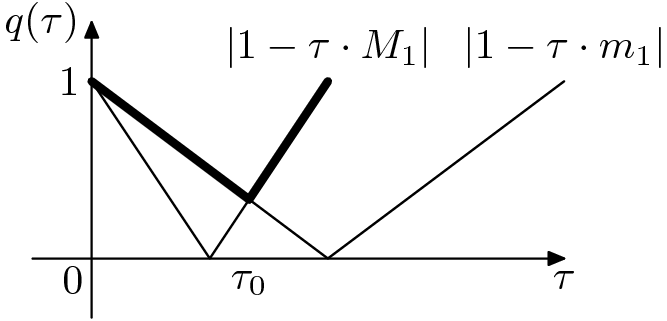
\includegraphics[width=.5\linewidth]{mal-1.png}
\end{figure}

% u:=1cm;
% label.llft(btex $0$ etex, (0,0));
% label.lft(btex $1$ etex, (0,3u/2));
% drawarrow (-u/2,0)--(4u,0);
% drawarrow (0,-u/2)--(0,2u);
% label.lft(btex $q(\tau)$ etex, (0,2u));
% label.bot(btex $\tau$ etex, (4u,0));
% draw (0,3u/2)--(u,0)--(2u,3u/2);
% draw (0,3u/2)--(2u,0)--(4u,3u/2);
% label.top(btex $|1-\tau \cdot M_1|$ etex, (2u,3u/2));
% label.top(btex $|1-\tau \cdot m_1|$ etex, (4u,3u/2));
% draw (4/3u,u/2)--(2u,3u/2) withpen pencircle scaled 2bp;
% draw (0,3u/2)--(4/3u,u/2) withpen pencircle scaled 2bp;
% label.bot(btex $\tau_0$ etex, (4/3u,0));

З графіка видно, що точка мінімуму визначається умовою $|1 - \tau \cdot M_1| = |1 - \tau \cdot m_1|$. \\

Тому
\[ 1 - \tau_0 \cdot m_1 = \tau_0 \cdot M_1 - 1 \Rightarrow \tau_0 = \dfrac{2}{M_1+m_1} < \dfrac{2}{|f'(x)|}.\]

При цьому значенні $\tau$ маємо \[q(\tau_0) = q_0 =\dfrac{M_1-m_1}{M_1+m_1}.\]

Тоді для похибки вірна оцінка \[|x_n-\overline{x}|\le \dfrac{q_0^n\cdot (b-a)}{1-q_0}<\epsilon.\]

Кількість ітерацій \[n = n(\epsilon) \ge \left\lfloor \dfrac{\ln \left(\dfrac{\epsilon\cdot(1-q_0)}{b-a}\right)}{\ln q_0} \right\rfloor + 1.\]	

\begin{problem} 
	Дати геометричну інтерпретацію методу простої ітерації для випадків:
	\[ 0 < \phi'(x) < 1; \quad -1 < \phi'(x) < 0; \quad \phi'(x) < -1; \quad \phi'(x) > 1,\]
\end{problem}

\begin{problem} 
	Знайти оптимальне $\tau = \tau_0$ для методу релаксації при $f'(x) > 0$.
\end{problem}

\subsection{Метод Ньютона (метод дотичних)}

Припустимо, що рівняння $f (x) = 0$ має простий дійсний корінь $\overline{x}$, тобто $f (\overline{x}) = 0$, $f'(\overline{x}) \ne 0$. Нехай виконуються умови: $f (x)\in C^{(1)}([a,b])$, $f (a)\cdot f (b) < 0$. Тоді 
\[0 = f (\overline{x}) = f (x_k + \overline{x} - x_k ) = f (x_k ) + f'(\xi_k ) \cdot (\overline{x} - x_k ),\] 
де $\xi_k=x_k+\theta_k \cdot (\overline{x}-x_k)$, $0 < \theta_k < 1$, $\xi_k \approx x_k$. Тому наступне наближення виберемо з рівняння 
\[ f(x_k) + f'(x_k) \cdot (x_{k+1}-x_k) = 0.\]

Звідси маємо ітераційний процес
\[ x_{k+1} = x_k - \dfrac{f(x_k)}{f'(x_k)}, \quad k = 0,1,2,\ldots, \quad x_0\text{ -- задане}. \]

Метод Ньютона ще називають методом лінеаризації або методом дотичних.

\begin{problem} 
	Дати геометричну інтерпретацію методу Ньютона.
\end{problem}

Метод Ньютона можна інтерпретувати як метод простої ітерації з \[ \phi(x) = x - \dfrac{f(x)}{f'(x)}, \quad \text{тобто} \quad \tau(x) = - \dfrac{1}{f'(x)}. \]

Тому 
\[ \phi'(x) = 1 - \dfrac{f'(x)\cdot f'(x)-f(x)\cdot f''(x)}{(f'(x))^2} = \dfrac{f(x)\cdot f''(x)}{(f'(x))^2}.\]
Якщо $\overline{x}$ -- корінь $f(x)$, то $\phi'(x) = 0$. Тому знайдеться окіл кореня, де \[ |\phi'(x)| = \left|\dfrac{f(x)\cdot f''(x)}{(f'(x))^2}\right|<1.\]

Це означає, що збіжність методу Ньютона залежить від вибору $x_0$. \\

Недолік методу Ньютона: необхідність обчислювати на кожній ітерації не тільки значення функції, а й похідної. \\

Модифікований метод Ньютона позбавлений цього недоліку і має вигляд:
\[ x_{k+1} = x_k - \dfrac{f(x_k)}{f'(x_0)}, \quad k=0,1,2,\ldots. \]

Цей метод має лише лінійну збіжність: $|x_{k+1} - \overline{x}| = O(|x_k-\overline{x}|)$.
\begin{problem} 
	Дати геометричну інтерпретацію модифікованого методу Ньютона.
\end{problem}

В методі Ньютона, для якого $f'(x_k)$ замінюється на $\frac{f(x_k)-f(x_{k-1})}{x_k-x_{k-1}}$ дає метод січних: \[ x_{k+1} = x_k - \dfrac{x_k-x_{k-1}}{f(x_k)-f(x_{k-1})}\cdot f(x_k), \quad k = 1,2,\ldots, \quad x_0,x_1\text{ -- задані}.\]

\begin{problem} 
	Дати геометричну інтерпретацію методу січних.
\end{problem}

\subsection{Збіжність методу Ньютона}

\begin{theorem}
	Нехай $f(x)\in C^{(2)}([a,b])$, $\overline{x}$ -- простий дійсний корінь рівняння
	\begin{equation}
		\label{eq:2.10}
		f (x) = 0
	\end{equation}
	і $f'(x) \ne 0$ при $x\in U_r= \{x: |x -\overline{x}| < r\}$. Якщо
	\begin{equation}
		\label{eq:2.11}
		\dfrac{M_2\cdot|x_0-\overline{x}|}{2m_1} = q < 1
	\end{equation}
	де $m_1 = \Min_{x\in U_r} |f'(x)|$, $M_2 = \Max_{x\in U_r} |f''(x)|$, то для $x_0 \in U_r$ метод Ньютона 
	\begin{equation}
		\label{eq:2.12}
		x_{k+1} = x_k - \dfrac{f(x_k)}{f'(x_k)}
	\end{equation}
	збігається і має місце оцінка
	\begin{equation}
		\label{eq:2.13}
		|x_n - \overline{x}| \le q^{2^n-1} \cdot |x_0 - \overline{x}|.
	\end{equation}
\end{theorem}

\begin{proof}
	З (\ref{eq:2.12}) маємо 
	\begin{equation}
		\label{eq:2.14}
		x_{k+1} - \overline{x} = x_k - \dfrac{f(x_k)}{f'(x_k)} - \overline{x} = \dfrac{(x_k-\overline{x}) \cdot f'(x_k)-f(x_k)}{f'(x_k)} = \dfrac{F(x_k)}{f'(x_k)},
	\end{equation}
	де $F(x) = (x - \overline{x}) \cdot f'(x) - f (x)$, така, що
	\begin{enumerate}
		\item $F(x) = 0$;
		\item $F'(x) = (x - \overline{x}) \cdot f''(x)$;
	\end{enumerate}
	Тоді \[ F(x_k) = F(\overline{x}) + \Int_{\overline{x}}^{x_k}  F'(t) \diff t = \Int_{\overline{x}}^{x_k}  ((t - \overline{x}) \cdot f''(t)) \diff t . \]

	Так як $(t - x)$ не міняє знак на відрізку інтегрування, то скористаємося теоремою про середнє значення:
	\begin{equation}
		\label{eq:2.15}
		F(x_k) = f''(\xi_k) \Int_{\overline{x}}^{x_k}  (t - \overline{x}) \diff t = \dfrac{(x_k-\overline{x})^2}{2} f''(\xi_k),
	\end{equation}
	де $\xi_k = \overline{x} + \theta_k \cdot (x_k - \overline{x})$, $0 <\theta_k < 1$. З (\ref{eq:2.14}), (\ref{eq:2.15}) маємо
	\begin{equation}
		\label{eq:2.16}
		x_{k+1} - \overline{x} = \dfrac{(x_k-\overline{x})^2}{2f'(x_k)} f''(\xi_k).
	\end{equation}
	Доведемо оцінку (\ref{eq:2.12}) за індукцією. Так як $x_0 \in U_r$, то \[|\xi_0 - \overline{x}| = |\theta_0 \cdot (x_0 - \overline{x})| < |\theta_0| \cdot |x_0 - \overline{x}| < r \Rightarrow \xi_0 \in U_r.\]

	Тоді $f''(\xi_0) \le M_2$, тому
	\begin{multline*} 
		|x_1 - \overline{x}| \le \dfrac{(x_0-\overline{x})^2 \cdot M_2}{2m_1} = \dfrac{M_2\cdot|x_0-\overline{x}|}{2m_1}|x_0-\overline{x}| = \\
		= q\cdot |x_0-\overline{x}|=q\cdot |x_0-\overline{x}|<r \Rightarrow x_1\in U_r.
	\end{multline*}

	Ми довели твердження (\ref{eq:2.13}) при $n = 1$. Нехай воно справджується при $n = k$:
	\[ |x_k - \overline{x}| \le q^{2^k-1}\cdot |x_0 - \overline{x}| < r, \quad |\xi_k - \overline{x}| = |\theta_k \cdot (x_k - \overline{x})| < r. \]

	Тоді $x_k, \xi_k \in U_r$. \\

	Доведемо (\ref{eq:2.13}) для $n = k +1$. З (\ref{eq:2.16}) маємо 
	\begin{multline*}
		|x_{k+1}-\overline{x}| \le \dfrac{|x_k - \overline{x}|^2\cdot M_2}{2m_1} \le \left(q^{2^k-1}\right)^2 \dfrac{|x_0-\overline{x}|^2\cdot M_2}{2m_1} = \\
		= q^{2^{k+1}-2} \dfrac{|x_0-\overline{x}|\cdot M_2}{2m_1}|x_0-\overline{x}| = q^{2^{k+1}-1} \cdot |x_0-\overline{x}|.
	\end{multline*}

	Таким чином (\ref{eq:2.13}) справджується для $n = k +1$. Значить (\ref{eq:2.13}) виконується і для довільного $n$. Таким чином $x_n \xrightarrow[n\to\infty]{} \overline{x}$.
\end{proof}

З (\ref{eq:2.13}) маємо оцінку кількості ітерацій для досягнення точності $\epsilon$:
\[ n \ge \left\lfloor\log_2\left(1+\dfrac{\ln \left(\dfrac{\epsilon}{b-a}\right)}{\ln q}\right) \right\rfloor + 1 .\]

Кажуть, що ітераційний метод має \textit{степінь збіжності} $m$, якщо \[ |x_{k+1}-\overline{x}|=O(|x_k-\overline{x}|^m).\]

Для методу Ньютона 
\[|x_{k+1}-\overline{x}| = \dfrac{|x_k-\overline{x}|^2\cdot|f''(\xi_k)|}{2|f'(x_k)|}| \Rightarrow |x_{k+1}-\overline{x}|=O(|x_k-\overline{x}|^2).\]

Значить степінь збіжності методу Ньютона $m=2$. Для методу простої ітерації і ділення навпіл $m=1$.

\begin{theorem}
	Нехай $f(x)\in C^{(2)}([a,b])$ та $\overline{x}$ -- простий корінь рівняння $f (x) = 0$ а також $\forall x\in[a,b]$: $f'(x) \ne 0$. Якщо $f'(x) \cdot f''(x) > 0$ ($f'(x) \cdot f''(x) < 0$) то для методу Ньютона при $x_0 = b$ послідовність наближень $\{x_k \}$ монотонно спадає (монотонно зростає при $x_0 = a$).
\end{theorem}

\begin{problem}
	Довести теорему при 
	\begin{enumerate}
		\item $f'(x) \cdot f''(x) > 0$;
		\item $f'(x) f''(x) < 0$.
	\end{enumerate}
\end{problem}

\begin{problem}
	Знайти степінь збіжності методу січних.
\end{problem}


Якщо $f(a) \cdot f''(a) > 0$ та $f''(x)$ не міняє знак, то потрібно вибирати $x_0 = a$; при цьому $\{x_k \}\uparrow \overline{x}$. \\

Якщо $f(b) \cdot f''(b) > 0$, то $x_0 = b$; маємо $\{x_k \}\downarrow \overline{x}$. Пояснення на рисунку:

% u := 1cm;
% drawarrow (-u/2, 0)--(4u, 0);
% drawarrow (0, -u/2)--(0, 2u);
% draw (u/2,0)--(u/2,u/8);
% draw (7u/2,0)--(7u/2,u/8);
% label.bot(btex $a$ etex, (u/2, 0));
% label.top(btex $b$ etex, (7u/2, u/8));
% draw (u/2,3u/2){dir -75}..(2u,-u/2){dir 0}..(7u/2,-u/4);
% label.top(btex $x_0 = a$ etex, (2u,u));

% u := 1cm;
% drawarrow (-u/2, 0)--(4u, 0);
% drawarrow (0, -u/2)--(0, 2u);
% draw (u/2,0)--(u/2,u/8);
% draw (7u/2,0)--(7u/2,u/8);
% label.top(btex $a$ etex, (u/2, u/8));
% label.bot(btex $b$ etex, (7u/2, 0));
% draw (u/2,-3u/7){dir 75}..(2u,u)..(7u/2,3u/2);
% label.top(btex $x_0 = a$ etex, (2u,3u/2));

\begin{figure}[H]
	\centering
	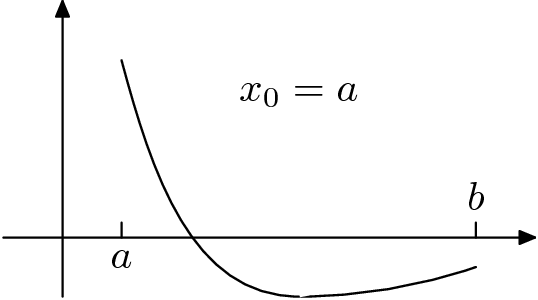
\includegraphics[width=.45\linewidth]{mal-2.png}
	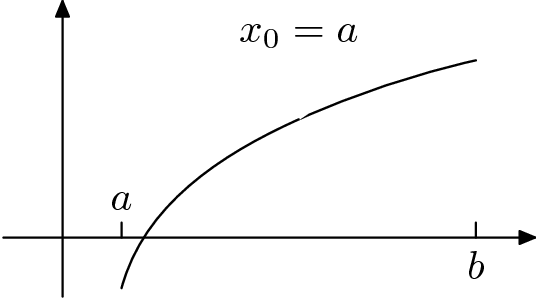
\includegraphics[width=.45\linewidth]{mal-3.png}
\end{figure}

\begin{remark}
	Якщо $\overline{x}$ -- $p$-кратний корінь тобто $f^{(m)} (x) = 0$, $m = \overline{0,p-1}$, $f^{ (p)} (x) \ne 0$, то в методі Ньютона необхідна наступна модифікація \[x_{k+1} = x_k - p\dfrac{f(x_k)}{f'(x_k)} \quad \text{і} \quad q = \dfrac{M_{p+1}\cdot|x_0-\overline{x}|}{m_p \cdot (p+1)}<1.\]
\end{remark}

\begin{remark}
Метод Ньютона можна застосовувати і для обчислення комплексного кореня, тоді ітераційний процес має вигляд \[z_{k+1} = z_k - \dfrac{f(z_k)}{f'(z_k)}, \quad k = 0,1,\ldots.\] В теоремі про збіжність $q = \frac{|z_0-\overline{z}|\cdot M_2}{2m_1}$, де $m_1 = \Min_{z\in U_r} |f'(z)|$, $M_2 = \Max_{z\in U_r} |f''(z)|$. Тут $|z|$ -- модуль комплексного числа $z$.
\end{remark}

Переваги методу Ньютона: 
\begin{enumerate}
\item висока швидкість збіжності;
\item узагальнюється на системи рівнянь; 
\item узагальнюється на комплексні корені.
\end{enumerate}
Недоліки методу Ньютона: 
\begin{enumerate}
	\item на кожній ітерації обчислюється не тільки $f (x_k )$ , а і похідна $f'(x_k)$;
	\item  збіжність залежить від початкового наближення $x_0$, так як від нього залежить умова збіжності $q = \frac{M_2\cdot |x_0-\overline{x}|}{2m_1} < 1$;
	\item потрібно, щоб $f (x)\in C^{(2)}([a,b])$.
\end{enumerate}
%\subsubsection{Характеристики розсіювання значень}
Нехай маємо вибірку об'єму $n$ спостережень $x_1$, $x_2$, $\ldots$, $x_n$ над випадковою величиною $\xi$.
\begin{enumerate}
	\item \textit{Дисперсія} $D\xi = M(\xi - M\xi)^2$. Вибіркове значення \[ S^2(n) = \dfrac{1}{n-1} \sum_{i=1}^n (x_i - \bar{x}(n))^2 = \dfrac{1}{n-1} \left(\sum_{i=1}^n x_i^2 - n\bar{x}^2(n) \right). \]
	\item \textit{Стандартне (середньоквадратичне) відхилення} $\sqrt{D\xi}$. Вибіркове значення $S(n)$.
	\item \textit{Коефіцієнт варіацій} $V_\xi = \frac{\sqrt{D\xi}}{M\xi} 100\%$, $M\xi\ne0$. Вибіркове значення $\widehat{V}_\xi(n)=\frac{S(n)}{\bar x(n)} 100\%$.
	\item \textit{Стохастичне розсіювання} (імовірнісне відхилення) -- це половина інтерквартильної широти: $\frac{U_{0.75} - U_{0.25}}{2}$. Вибіркове значення $\frac{\widehat{U}_{0.75} - \widehat{U}_{0.25}}{2}$.
	\item \textit{Розмах (широта) вибірки}: $x_{\max}-x_{\min}$, де $x_{\max}, x_{\min}$ -- найбільше та найменше значення у вибірці.
	\item \textit{Інтервал концентрації} $(M\xi - 3\sqrt{D\xi}, M\xi + 3 \sqrt{D\xi})$. Вибіркове значення $(\bar x(n) - 3S(n), M\bar x(n) + 3 S(n))$.
\end{enumerate}
\subsubsection{Характеристики скошеності та гостроверхості розподілу}
Нехай є розподіл випадкової величини $\xi$ і отримані спостереження $x_1$, $x_2$, $\ldots$, $x_n$ над нею.
\begin{enumerate}
	\item \textit{Коефіцієнт асиметрії} -- характеристика скошеності розподілу (базується на третьому центральному моменті): \[ \beta_1 = \dfrac{M(\xi - M\xi)^3}{(M(\xi - M\xi)^2)^{3/2}}, \quad D\xi > 0. \] Вибіркове значення \[ \widehat{\beta}_1 = \dfrac{\dfrac{1}{n}\Sum_{i=1}^n(x_k - \bar{x}(n))^3}{S^3(n)}. \] Дисперсія спостережуваної величини $D\xi > 0$. \\ % figure 6

	Якщо розподіл симетричний (наприклад нормальний) то $\beta_1 =0$. Якщо $\beta_1 > 0$, то розподіл скошений вліво, якщо $\beta_1 < 0$, то вправо.
	\item \textit{Коефіцієнт ексцесу} -- характеристика гостроверхості розподілу (базується на четвертому центральному моменті): \[ \beta_2 = \dfrac{M(\xi-M\xi)^4}{(M(\xi-M\xi)^2)^2} - 3, \quad D\xi > 0. \] Вибіркове значення \[ \widehat{\beta}_2 = \dfrac{\dfrac{1}{n}\Sum_{i=1}^n(x_k - \bar{x}(n))^4}{S^4(n)} - 3. \]
	Для нормального розподілу коефіцієнт ексцесу дорівнює нулю. Якщо $\beta_2 > 0$, то розподіл більш гостроверхий ніж нормальний, якщо $\beta_2 < 0$ то відповідно менш гостроверхий.
\end{enumerate}
\subsection{Характеристики векторних величин}
Аналіз $q$-вимірних векторних величин, отримано $n$ спостережень над вектором $\vec\xi: x_1, x_2, \ldots, x_n$, $x_i \in \RR^q$, $i = \overline{1,n}$.
\subsubsection{Характеристики положення центру значень}
\begin{enumerate}
	\item \textit{Математичне сподівання} (теоретичне середнє) $M\xi$. Вибіркове значення \[\bar{x}(n) = \dfrac{1}{n} \Sum_{i=1}^n \vec{x}_i.\]
	\item \textit{Мода} $x_{\text{mod}}$. У неперервному випадку -- це точка максимуму функції щільності $\xi$. Для дискретного випадку -- це значення, яке набуває $\xi$ з найбільшою ймовірністю.
\end{enumerate}
\subsubsection{Характеристики розсіювання значень}
\begin{enumerate} 
	\item \textit{Коваріаційна матриця} $\sum = M(\xi - M\xi)(\xi - M\xi)^T$. Вибіркове значення \[\widehat{\sum}(n) = \dfrac{1}{n-1} \Sum_{k=1}^n (x_k - \bar x(n))(x_k - \bar x(n))^T.\]
	\item \textit{Узагальнена дисперсія} -- визначник коваріаційної матриці: $\det \sum$. Вибіркове значення $\det\left(\widehat{\sum}\right)$.
	\item \textit{Слід коваріаційної матриці} $\trace\sum$. Вибіркове значення $\trace\left(\widehat{\sum}(n)\right)$.
\end{enumerate}
\subsection{Перевірка стохастичності вибірки}
Перевіряємо, чи справді вибірка є випадковою, а не знаходиться під впливом деякого систематичного зміщення. Для цього запропоновано критерії:
\begin{itemize}
	\item Критерій серій на базі медіани
	\item Критерій зростаючих та спадаючих серій
	\item Критерій квадратів послідовних різниць (критерій Аббе)
\end{itemize}
Нехай $x_1$, $x_2$, $\ldots$, $x_n$ -- вибірка спостережень, яка досліджується. \\

Будемо перевіряти гіпотезу $H_0$: ця вибірка є стохастичною з рівнем значимості $\alpha (0 < \alpha < 1$) (рівень значимості -- ймовірність допустити помилку першого роду).
\begin{enumerate}
	\item \textit{Критерій серій на базі медіани}. Альтернативна гіпотеза $H_1$: наявність у вибірці систематичного монотонного зміщення середнього. \\

	Спочатку визначається вибіркове значення медіани $\widehat{x}_{\text{med}}$. Потім під кожним членом вибірки ставимо відповідно \[ \begin{cases} +, & x_i > \widehat{x}_{\text{med}} \\
 \text{нічого}, & x_i = \widehat{x}_{\text{med}} \\
 -, & x_i < \widehat{x}_{\text{med}} \end{cases}. \]
	Отримаємо послідовність символів. \textit{Серія} -- послідовність підряд розташованих однакових символів $+$ чи $-$. \textit{Довжина серії} -- це кількість членів у ній. \\

	Для отриманої послідовності обчислюємо дві статистики: загальну кількість серій в послідовності $v(n)$, довжину найдовшої серії $\tau(n)$. Запишемо область прийняття нашої гіпотези: \[ \left\{ \begin{matrix} v(n) > v_\beta(n) \\
 \tau(n) < \tau_{1-\beta}(n) \end{matrix} \right. \] 
	де $v_\beta(n)$, $\tau_\beta(n)$ -- квантилі рівня $\beta$ статистик $v(n)$, $\tau(n)$ відповідно. При фіксованому значенні $\beta$ рівень значимості $\alpha$ лежить у межах $\beta < \alpha < 2\beta - \beta^2$. Якщо порушується хоч одна з нерівностей, то гіпотеза відхиляється.
	\item \textit{Критерій зростаючих та спадаючих серій}. Альтернативна гіпотеза $H_1$: наявність у вибірці систематичного періодичного зміщення середнього. Спочатку у вибірці замінюємо підряд розташовані однакові виміри одним їх представником. В результаті отримаємо послідовність $x_1'$, $x_2'$, $\ldots$, $x_k'$. Під кожним членом послідовності ставимо відповідно \[ \begin{cases} +, & x_i' < x_{i+1}' \\
 -, & x_i' > x_{i+1}' \end{cases}. \]
	Далі для таким чином отриманої послідовності $+$ та $-$, як і в попередньому випадку, обчислюємо дві статистики: загальну кількість серій в послідовності $v(n)$, довжину найдовшої серії $\tau(n)$. Запишемо область прийняття нашої гіпотези: \[ \left\{ \begin{matrix} v(n) > v_\beta(n) \\
 \tau(n) < \tau_{1-\beta}(n) \end{matrix} \right. \] де $v_\beta(n)$, $\tau_\beta(n)$ -- квантилі рівня $\beta$ статистик $v(n)$, $\tau(n)$ відповідно. При фіксованому значенні $\beta$ рівень значимості $\alpha$ лежить у межах $\beta < \alpha < 2\beta - \beta^2$. Якщо порушується хоч одна з нерівностей, то гіпотеза відхиляється.
	\item \textit{Критерій квадратів послідовних різниць (критерій Аббе)}. Він є найбільш потужним на класі усіх нормальних вибірок. Альтернативна гіпотеза $H_1$: наявність у вибірці систематичного зміщення середнього. \\

	На основі вибірки підраховуємо наступну статистику: \[ \gamma(n) = \dfrac{\dfrac{1}{2(n-1)} \Sum_{i=1}^{n-1} (x_{i+1}-x_i)^2}{\dfrac{1}{n-1}\left(\Sum_{i=1}^n x_i^2 - n \bar{x}^2(n)\right)}. \]
	Область прийняття гіпотези для цього критерію має вигляд $\gamma(n) > \gamma_\alpha(n)$, де $\gamma_\alpha(n)$ -- квантиль рівня $\alpha$ статистики $\gamma(n)$, що при $n \le 60 $визначається з таблиць, а протилежному випадку потрібно скористатися формулою \[\gamma_\alpha(n) = 1 + \dfrac{u_\alpha}{\sqrt{n + 0.5(1 + u_\alpha^2)}}, \] де $u_\alpha$ -- квантиль рівня $\alpha$ нормального розподілу з параметрами 0 та 1.
\end{enumerate}

 \setcounter{section}{2}
 \setcounter{subsection}{3}
 \setcounter{subsubsection}{0}
 \setcounter{theorem}{14}
 \setcounter{equation}{4}

\subsubsection{Характеристичні числа ермітового неперервного ядра}

\begin{theorem}[про існування характеристичного числа у ермітового неперервного ядра]
	Для будь-якого ермітового неперервного ядра, що не дорівнює тотожно нулю існує принаймні одне характеристичне число і найменше з них за модулем $\lambda_1$ задовольняє варіаційному принципу
	\begin{equation}
		\dfrac{1}{|\lambda_1|} = \Sup_{f \in L_2(G)} \dfrac{\|\bf{K} f\|_{L_2(G)}}{\|f\|_{L_2(G)}}.
	\end{equation}
\end{theorem}

\begin{proof}
	Серед усіх $f \in L_2$ оберемо такі, що $\|f\|_{L_2(G)} = 1$. Позначимо 
	\begin{equation}
		\nu = \Sup_{\substack{f \in L_2(G) \\ \|f\|_{L_2} = 1}} \|\bf{K} f\|_{L_2(G)}.
	\end{equation}
	
	Оскільки
	\begin{equation}
		\|\bf{K} f\|_{L_2(G)} \le MV \|f\|_{L_2(G)} \le MV,
	\end{equation}


	Згідно до визначення точної верхньої межі,
	\begin{equation}
		\exists \{ f_k \}_{k = 1}^\infty \subset L_2(G):\lim_{n \to \infty} \|\bf{K} f_k\|_{L_2(G)} = \nu.
	\end{equation}

	Оцінимо 
	\begin{equation}
		\begin{aligned} 
		\left\| \bf{K}^2 f\right\|_{L_2(G)} &= \| \bf{K} (\bf{K} f)\|_{L_2(G)} = \\
		&=  \left\| \bf{K}\left( \dfrac{\bf{K}f}{\|\bf{K}f\|}\right) \right\|_{L_2(G)} \cdot \|\bf{K} f\|_{L_2(G)} \le \\
		&\le  \nu \cdot \|\bf{K} f\|_{L_2(G)} \le \nu^2.
		\end{aligned}
	\end{equation}
	
	Покажемо, що $\bf{K}^2 f_k - \nu^2 f_k \to 0$ в середньому квадратичному. Тобто що
	\begin{equation}
		\| \bf{K}^2 f_k - \nu^2 f_k \|_{L_2(G)}^2 \xrightarrow[k \to \infty]{} 0.
	\end{equation}

	Дійсно:
	\begin{equation}
		\begin{aligned}
			\| \bf{K}^2 f_k - \nu^2 f_k \|_{L_2(G)}^2 &= (\bf{K}^2 f_k - \nu^2 f_k, \bf{K}^2 f_k - \nu^2 f_k)_{L_2(G)} = \\
			&= \|\bf{K}^2 f_k\|_{L_2(G)}^2 + \nu^4 - \nu^2 (\bf{K}^2 f_k, f_k) - \nu^2 (f_k, \bf{K}^2 f_k) = \\
			&= \|\bf{K}^2 f_k\|_{L_2(G)}^2 + \nu^4 - 2 \nu^2 \|\bf{K} f_k\|_{L_2(G)}^2 \le \\
			&\le \nu^2 \left(\nu^2 - \|\bf{K}^2 f_k\|_{L_2(G)}^2\right) \xrightarrow[k\to\infty]{} 0.
		\end{aligned}
	\end{equation}

	Розглянемо послідовність $\{ \bf{K}f_k \} = \{ \phi_k\}$, яка є компактною в рівномірній метриці. \medskip

	У неї існує підпослідовність $\{\phi_{k_i}\}_{i = 1}^\infty$ збіжна в $C\left(\overline G\right)$, тобто $\exists \phi \in C\left(\overline G\right)$, така що $\| \phi_{k_i} - \phi\|_{C\left(\overline G\right)} \xrightarrow[i \to \infty]{} 0$. \medskip

	Покажемо, що $\bf{K}^2 \phi - \nu^2 \phi = 0$ в кожній точці, тобто $\| \bf{K}^2\phi - \nu^2 \phi\|_{C\left(\overline G\right)} = 0$. \medskip

	Справді,
	\begin{equation}
		\begin{aligned}
			\|\bf{K}^2\phi - \nu^2\phi\|_{C\left(\overline G\right)} &= \|\bf{K}^2\phi - \bf{K}^2\phi_{k_i} + \bf{K}^2\phi_{k_i} - \nu^2\phi_{k_i} + \nu^2\phi_{k_i} - \nu^2\phi\|_{C\left(\overline G\right)} \le \\
			&\le \|\bf{K}^2\phi-\bf{K}^2\phi_{k_i}\|_{C\left(\overline G\right)} + \|\bf{K}^2\phi_{k_i}-\nu^2\phi_{k_i}\|_{C\left(\overline G\right)}+ \\
			&\quad + \|\nu^2\phi_{k_i}-\nu^2\phi\|_{C\left(\overline G\right)} \le \\
			&\le (MV)^2 \|\phi_{k_i} - \phi\|_{C\left(\overline G\right)} + M\sqrt{V} \|\bf{K}^2f_{k_i}-\nu^2f_{k_i}\|_{L_2(\overline G)} + \\
			&\quad + \nu^2 \|\phi_{k_i} - \phi\|_{C\left(\overline G\right)} \to 0 + 0 + 0.
		\end{aligned}
	\end{equation}
	
	Таким чином має місце рівність
	\begin{equation}
		\bf{K}^2 \phi - \nu^2 \phi = 0
	\end{equation}
	
	Отже маємо: $(\bf{K} + E\nu)(\bf{K} - E \nu)\phi=0$. Ця рівність може мати місце у двох випадках:
	\begin{enumerate}
		\item $(\bf{K} - E\nu) \phi \equiv 0$. Тоді $\phi = \frac{1}{\nu}\bf{K}\phi$, а отже $\phi$ --- власна функція, $\frac{1}{\nu}$ --- характеристичне число оператора $\bf{K}$.

		\item $(\bf{K} - E\nu) \phi \equiv \Phi \ne 0$. Тоді $(\bf{K} + E \nu) \Phi \equiv 0$. Тоді $\Phi = -\frac{1}{\nu}\bf{K}\Phi$, а отже $\Phi$ --- власна функція, $-\frac{1}{\nu}$ --- характеристичне число оператора $\bf{K}$.
	\end{enumerate}
	
	Залишилось довести, що це характеристичне число є мінімальним за модулем. Припустимо супротивне. Нехай $\exists \lambda_0: |\lambda_0| < |\lambda_1|$, тоді
	\begin{equation}
		\frac{1}{|\lambda_1|} = \sup_{f \in L_2(G)} \frac{\|\bf{K}f\|}{\|f\|} \ge \frac{\|\bf{K}\phi_0\|}{\|\phi_0\|} = \frac{1}{|\lambda_0|},
	\end{equation}
	тобто $|\lambda_0| \ge |\lambda_1|$, протиріччя.
\end{proof}

\begin{remark}
	Доведена теорема є вірною і для ермітових полярних ядер,
\end{remark}

Звідси безпосередньо випливають такі 
\begin{properties}[характеристичних чисел та власних функцій ермітового ядра]
	Нескладно показати, що:
	\begin{enumerate}
		\item Множина характеристичних чисел ермітового неперервного \allowbreak ядра не порожня, є підмножиною множини дійсних чисел і не має скінчених граничних точок.
		\item Кратність будь-якого характеристичного числа скінчена.
		\item Власні функції можна вибрати так, що вони утворять ортонормовану систему, тобто $\{ \phi_k\}_{k = 1, 2, \ldots}$ такі що $(\phi_k, \phi_i)_{L_2(G)} = \delta_{ki}$.
	\end{enumerate}
\end{properties}

\begin{remark}
	Для доведення останньої властивості достатньо провести процес ортогоналізації Гілберта-Шмідта для будь-якої системи лінійно незалежних власних функцій, і пронормувати отриману систему.
\end{remark}

\subsection{Теорема Гілберта-Шмідта та її наслідки}

\subsubsection{Білінійе розвинення ермітового неперервного ядра}

Нехай $K(x, y) \in C\left(\overline G \times \overline G\right)$ --- ермітове неперервне ядро, $|\lambda_i| \le |\lambda_{i + 1}|$, $i = 1, 2, \ldots$ --- його характеристичні числа і $\{\phi_i\}_{i = 1}^\infty$ --- ортонормована система власних функцій, що відповідають власним числам. \medskip

Розглянемо послідовність ермітових неперервних ядер:
\begin{equation}
	K^p(x, y) = K(x, y) - \Sum_{i = 1}^p \dfrac{\overline \phi_i(y) \phi_i(x)}{\lambda_i}, \quad p = 1, 2, \ldots
\end{equation}

Зрозуміло що при цьому
\begin{equation}
	K^p(x, y) = (K^p)^\star (x, y) \in  C\left(\overline G \times \overline G\right).
\end{equation}

Дослідимо властивості  ермітових операторів, що відврвідають ядру $K^p(x, y)$.

\begin{proposition}
	Будь-яке характеристичне число $\lambda_j$, $j >= p + 1$ та відповідна йому власна функція $\phi_j$ є характеристичним числом і власною функцією ядра $K^p(x,y)$.
\end{proposition}

\begin{proof}
	Справді:
	\begin{equation}
		\bf{K}^p \phi_j = \bf{K} \phi_j - \Sum_{i = 1}^p \dfrac{\phi_i(x)}{\lambda_i} (\phi_i, \phi_j) = \bf{K} \phi_j = \dfrac{\phi_j}{\lambda_j}.
	\end{equation}
\end{proof}

Нехай $\lambda_0$, $\phi_0$ --- характеристичне число та відповідна власна функція $K^p(x, y)$, тобто $\lambda_0 \bf{K}^p \phi_0 = \phi_0$.

\begin{proposition}
	$(\phi_0, \phi_j) = 0$ для $j = \overline{1, p}$.
\end{proposition}

\begin{proof}
	З того, що $\phi_0$ є власною функцією ядра $\bf{K}^p$ випливає, що
	\begin{equation}
		\phi_0 = \lambda_0 \bf{K} \phi_0 - \lambda_0 \Sum_{i = 1}^p \dfrac{\phi_i}{\lambda_i} (\phi_0, \phi_i).
	\end{equation}

	Підставляючи цей вираз для $\phi_0$ у потрібний скалярний добуток маємо
	\begin{equation}
		\begin{aligned}
			(\phi_0, \phi_j) &= \lambda_0 (\bf{K} \phi_0, \phi_j) - \lambda_0 \Sum_{i = 1}^p \dfrac{(\phi_0, \phi_i)(\phi_i, \phi_j)}{\lambda_i} = \\
			&= \dfrac{\lambda_0}{\lambda_j} (\phi_0, \phi_j) - \dfrac{\lambda_0}{\lambda_j} (\phi_0, \phi_j) = 0. 
		\end{aligned}
	\end{equation}
\end{proof}

Отже $\lambda_0$, $\phi_0$ відповідно характеристичне число і власна функція ядра $K(x, y)$. \medskip

Таким чином $\phi_0$ --- ортогональна до усіх власних функцій $\phi_1$, $\phi_2$, $\ldots$, $\phi_p$. Але тоді $\lambda_0$ співпадає з одним із характеристичних чисел $\lambda_{p + 1}$, $\lambda_{p + 2}$, $\ldots$ тобто $\phi_0 = \phi_k$ для деякого $k \ge p + 1$. \medskip

Отже у ядра $K^p(x, y)$ множина власних функцій і характеристичних чисел вичерпується множиною власних функцій і характеристичних чисел ядра $K(x, y)$ починаючи з номера $p + 1$. \medskip

Враховуючи, що $\lambda_{p + 1}$ --- найменше за модулем характерне число ядра $K^p(x, y)$, має місце нерівність
\begin{equation}
	\dfrac{\|\bf{K}^p f\|_{L_2(G)}}{\|f\|_{L_2(G)}} \le \dfrac{1}{|\lambda_{p + 1}|}.
\end{equation}

Для ядра, що має скінчену кількість характеристичних чисел, очевидно, має місце рівність
\begin{equation}
	K^N(x, y) = K(x, y) - \sum_{i = 1}^N \frac{\phi_i(x) \overline \phi_i(y)}{\lambda_i} \equiv 0.
\end{equation}

Тобто будь-яке ермітове ядро зі скінченою кількістю характеристичних чисел є виродженим і представляється у вигляді
\begin{equation}
	K(x, y) = \sum_{i = 1}^N \frac{\phi_i(x) \overline \phi_i(y)}{\lambda_i}.
\end{equation}

Враховуючи теорему про існування характеристичних чисел у ермітового оператора можемо записати:
\begin{equation}
	\| K^{(p)} f \|_{L_2(G)} = \left\| \bf{K}f - \Sum_{i = 1}^p \dfrac{(f, \phi_i)}{\lambda_i} \phi_i \right\|_{L_2(G)} \le \dfrac{\|f\|_{L_2(G)}}{|\lambda_{p + 1}|} \xrightarrow[p\to\infty]{} 0.
\end{equation}

Тобто можна вважати, що ермітове ядро в певному розумінні наближається наступним білінійним рядом:
\begin{equation}
	K(x, y) \sim \Sum_{i = 1}^\infty \dfrac{\phi_i(x) \overline \phi_i(y)}{\lambda_i}.
\end{equation}

Для виродженого ядра маємо його представлення у вигляді
\begin{equation}
	K(x, y) = \Sum_{i = 1}^N \dfrac{\phi_i(x) \overline \phi_i(y)}{\lambda_i}.
\end{equation}

\subsubsection{Ряд Фур'є функції із $L_2(G)$}

Розглянемо довільну функцію $f \in L_2(G)$ і деяку ортонормовану систему функцій $\{ u_i \}_{i = 1}^\infty$. 

\begin{definition}[ряда Фур'є]
	\it{Рядом Фур'є} функції $f$ із $L_2(G)$ називається
	\begin{equation}
		\Sum_{i = 1}^\infty (f, u_i) u_i \sim f.
	\end{equation}
\end{definition}

\begin{definition}[коефіцієнта Фур'є]
	Вираз $(f, u_i)$ називається \it{коефіцієнтом Фур'є}.
\end{definition}

\begin{theorem}[нерівність Бесселя]
	$\forall f \in L_2(G)$ виконується \it{нерівність Бесселя}: $\forall N$
	\begin{equation}
		\Sum_{i = 1}^N |(f, u_i)|^2 \le \|f\|_{L_2(G)}^2.
	\end{equation}
\end{theorem}

\begin{remark}
	Нерівність Бесселя гарантує збіжність ряду Фур'є в середньоквадратичному, але не обов'язково до функції $f$.
\end{remark}

\begin{definition}[повної (замкненої) системи функцій]
	Ортонормована система функцій $\{ u_i \}_{i = 1}^\infty$ називається \it{повною (замкненою)}, якщо ряд Фур'є для будь-якої функції $f \in L_2(G)$ по цій системі функцій збігається до цієї функції в просторі $L_2(G)$.
\end{definition}

\begin{theorem}[критерій повноти ортонормованої системи функцій]
	Для того щоб система функцій $\{ u_i \}_{i = 1}^\infty$ була повною в $L_2(G)$ необхідно і достатньо, щоби для будь-якої функції $f \in L_2(G)$ виконувалась рівність Парсеваля-Стеклова:
	\begin{equation}
		\Sum_{i = 1}^\infty |(f, u_i)|^2 = \|f\|_{L_2(G)}^2.
	\end{equation}
\end{theorem}

\subsubsection{Теорема Гільберта-Шмідта}

\begin{definition}[джерелувато-зображуваної функції]
	Функція $f(x)$ називається \it{джерелувато-зображуваною} через ермітове неперервне ядро $K(x, y) = K^\star (x, y)$, $K \in  C\left(\overline G \times \overline G\right)$, якщо існує функція $h(x) \in L_2(G)$, така що 
	\begin{equation}
		f(x) = \Int_G K(x, y) h(y) \diff y.
	\end{equation}
\end{definition}

\begin{theorem}[Гільберта-Шмідта]
	Довільна джерелувато-зображувана функція $f$ розкладається в абсолютно і рівномірно збіжний ряд Фур'є за системою власних функцій ермітового неперервного ядра $K(x, y)$
\end{theorem}

\begin{proof}
	Обчислимо коефіцієнти Фур'є:
	\begin{equation}
		(f, \phi_i) = (\bf{K}h, \phi_i) = (h, \bf{K}\phi_i) = \frac{(h,\phi_i)}{\lambda_i}.
	\end{equation}

	Отже ряд Фур'є функції $f$ має вигляд 
	\begin{equation}
		f \sim \Sum_{i = 1}^\infty \dfrac{(h, \phi_i)}{\lambda_i} \phi_i
	\end{equation}

	Якщо власних чисел скінчена кількість, то можливе точне представлення 
	\begin{equation}
		f(x) = \sum_{i=1}^N \frac{(h, \phi_i)}{\lambda_i} \phi_i(x),
	\end{equation}
	якщо ж власних чисел злічена кількість, то  можемо записати:
	\begin{equation}
		\left\| f - \Sum_{i = 1}^p \dfrac{(h, \phi_i)}{\lambda_i} \phi_i \right\|_{L_2(G)} = \left\| \bf{K}h - \Sum_{i = 1}^p \dfrac{(h, \phi_i)}{\lambda_i} \phi_i \right\|_{L_2(G)} \xrightarrow[p \to \infty]{}0.
	\end{equation}
	Покажемо, що формулу 
	\begin{equation}
		K(x, y) \sim \Sum_{i = 1}^\infty \dfrac{\phi_i(x) \overline \phi_i(y)}{\lambda_i}.
	\end{equation}
	можна розглядати як розвинення ядра $K(x, y)$ в ряд Фур'є по системі власних функцій $\phi_i(x)$. Перевіримо це обчислюючи коефіцієнт Фур'є:
	\begin{equation}
		\begin{aligned}
			(K(x, y),\phi_i)_{L_2(G)} &= \Int_G K(x, y) \overline \phi_i(x) \diff x = \\
			&= \Int_G \overline {K(y, x)} \overline \phi_i(x) \diff x = \dfrac{\overline \phi_i(y)}{\lambda_i}.
		\end{aligned}
	\end{equation}

	Доведемо рівномірну збіжність ряду Фур'є за критерієм Коші і покажемо, що при, $n, m \to \infty$, відрізок ряду прямує до нуля. За нерівністю Коші-Буняківського маємо:
	\begin{equation}
		\left| \Sum_{i = n}^m \dfrac{(h, \phi_i)}{\lambda_i} \phi_i \right| \le \Sum_{i = n}^m |(h, \phi_i)\dfrac{|\phi_i|}{|\lambda_i|} \le \left(\Sum_{i=n}^m |(h, \phi_i)|^2\right)^{1/2} \cdot \left(\Sum_{i=n}^m \dfrac{|\phi_i|^2}{\lambda_i^2}\right)^{1/2}
	\end{equation}

	Але
	\begin{equation}
		\Sum_{i=n}^m |(h, \phi_i)|^2 \le \|h\|_{L_2(G)}^2,
	\end{equation}
	тобто ряд збігається, а вказана сума прямує до 0 при $n, m \to \infty$.

	Зокрема маємо
	\begin{equation}
		\Sum_{i=n}^m \dfrac{|\phi_i|^2}{\lambda_i^2} \le \Int_G |K(x, y)|^2 \diff x \le M^2 V, 
	\end{equation}
	тобто ряд збігається. \medskip

	Отже
	\begin{equation}
		\left(\Sum_{i=n}^m |(h, \phi_i)|^2\right)^{1/2} \left(\Sum_{i=n}^m \dfrac{|\phi_i|^2}{\lambda_i^2}\right)^{1/2} \xrightarrow[n, m \to \infty]{} 0,
	\end{equation}
	а отже
	\begin{equation}
		\sum_{i=1}^\infty \frac{(h, \phi_i)}{\lambda_i} \phi_i
	\end{equation}
	збігається абсолютно і рівномірно саме до функції $f(x)$.
\end{proof}

\begin{corollary}
	\label{corollary:2.4.10}
	Довільне повторне ядро для ермітового неперервного ядра $K(x ,y)$ розкладається в білінійний ряд по системі власних функцій ермітового неперервного ядра, який збігається абсолютно і рівномірно, а саме рядом
	\begin{equation}
		K_{(p)}(x, y) = \Sum_{i = 1}^\infty \dfrac{\phi_i(x) \overline \phi_i(y)}{\lambda_i^p},
	\end{equation}
	де $p = 2, 3, \ldots$, і коефіцієнти Фур'є  $\overline \phi_i(y) / \lambda_i^p$.
\end{corollary}

Повторне ядро $K_{(p)}(x,y) = \int_G K(x, \xi) K_{(p - 1)} (\xi, y) \diff \xi$ є джерелувато-зображувана функція і таким чином для нього має місце теорема Гільберта-Шмідта. \medskip

Доведемо деякі важливі рівності:
\begin{equation}
	\begin{aligned}
	K_{(2)} (x, x) &= \Int_G K(x, \xi) K(\xi, x) \diff \xi = \\
	&= \Int_G K(x, \xi) \overline {K(x, \xi)} \diff \xi = \\
	&= \Int_G |K(x, \xi)|^2 \diff \xi = \\
	&= \Sum_{i = 1}^\infty \dfrac{|\phi_i(x)|^2}{\lambda_i^2}.
	\end{aligned}
\end{equation}

\begin{remark}
	Останій перехід випливає з наслідку вище.
\end{remark}

Проінтегруємо отримане співвідношення, отримаємо
\begin{equation}
	\Iint_{G \times G} |K(x, y)|^2 \diff x \diff y = \Sum_{i = 1}^\infty \dfrac{1}{\lambda_i^2}.
\end{equation}

\begin{theorem}[про збіжність білінійного ряду для ермітового неперервного ядра]
	Ермітове неперервне ядро $K(x, y)$ розкладається в білінійний ряд
	\begin{equation}
		K(x, y) = \sum_{i=1}^\infty \frac{\phi_i(x) \overline \phi_i(y)}{\lambda_i}
	\end{equation}
	по своїх власних функціях, і цей ряд збігаються в нормі $L_2(G)$ по аргументу $x$ рівномірно для кожного $y \in \overline G$, тобто 
	\begin{equation}
		\left\| K(x, y) - \Sum_{i=1}^p \dfrac{\phi_i(x)\overline \phi_i(y)}{\lambda_i}\right\|_{L_2(x \in G)} \xrightrightarrows[p \to \infty]{y \in \overline G} 0.
	\end{equation}
\end{theorem}

\begin{proof}
	\begin{equation}
		\left\| K(x, y) - \Sum_{i = 1}^p \dfrac{\phi_i(x) \overline \phi_i(y)}{\lambda_i} \right\|_{L_2(G)}^2 = \Int_G |K(x, y)|^2 \diff x - \Sum_{i = 1}^p \dfrac{|\phi_i(y)|^2}{\lambda_i^2} \xrightrightarrows[p \to \infty]{y \in \overline G} 0.
	\end{equation}

	Додатково інтегруючи по аргументу $y \in G$ отримаємо збіжність вищезгаданого білінійного ряду в середньоквадратичному:
	\begin{equation}
		\Iint_{G \times G} \left( K(x, y) - \Sum_{i = 1}^p \dfrac{\phi_i(x) \overline \phi_i(y)}{\lambda_i} \right)^2 \diff y \diff x\xrightarrow[p \to \infty]{} 0.
	\end{equation}
\end{proof}

\subsubsection{Формула Шмідта для розв'язання інтегральних рівнянь з ермітовим неперервним ядром}

Розглянемо інтегральне рівняння Фредгольма 2 роду $\phi = \lambda \bf{K} \phi + f$, з ермітовим неперервним ядром 
\begin{equation} 
	K(x, y) = K^\star  (x, y).
\end{equation}
$\lambda_1, \ldots, \lambda_p, \ldots$, $\phi_1, \ldots, \phi_p, \ldots$ --- множина характеристичних чисел та ортонормована система власних функцій ядра $K(x, y)$. \medskip

Розкладемо розв'язок рівняння $\phi$ по системі власних функцій ядра $K(x, y)$:
\begin{equation}
	\begin{aligned}
		\phi &= \lambda \Sum_{i = 1}^\infty (\bf{K}\phi, \phi_i) \phi_i + f = \\
		&= \lambda \Sum_{i = 1}^\infty (\phi, \bf{K} \phi_i) \phi_i + f = \\
		&= \lambda \Sum_{i = 1}^\infty \dfrac{(\phi, \phi_i)}{\lambda_i} \phi_i + f,
	\end{aligned}
\end{equation}

Обчислимо коефіцієнти Фур'є:
\begin{equation}
	(\phi, \phi_k) = \lambda \Sum_{i = 1}^\infty \dfrac{(\phi, \phi_i)}{\lambda_i} (\phi_i, \phi_k) + (f, \phi_k) = \lambda \dfrac{(\phi, \phi_k)}{\lambda_k} + (f, \phi_k).
\end{equation}

Отже,
\begin{equation}
	(\phi, \phi_k) \left(1 - \frac{\lambda}{\lambda_k}\right) = (f, \phi_k),
\end{equation}
і тому
\begin{equation}
	(\phi, \phi_k) = (f, \phi_k) \frac{\lambda_k}{\lambda_k - \lambda}, \quad k = 1, 2, \ldots
\end{equation}

Таким чином має місце 
\begin{theorem}[формула Шмідта]
	Виконується співвідношення
	\begin{equation}
		\phi(x) = \lambda \Sum_{i = 1}^\infty \dfrac{(f, \phi_i)}{\lambda_i - \lambda} \phi_i(x) + f(x).
	\end{equation}
\end{theorem}

Розглянемо усі можливі значення $\lambda$:
\begin{enumerate}
	\item Якщо $\lambda \notin \{\lambda_i\}_{i=1}^\infty$, тоді існує єдиний розв'язок для довільного вільного члена $f$ і цей розв'язок представляється за формулою Шмідта.
	
	\item Якщо $\lambda = \lambda_k = \lambda_{k + 1} = \ldots = \lambda_{k + q - 1}$ --- співпадає з одним з характеристичних чисел кратності $q$, та при цьому виконуються умови ортогональності
	\begin{equation}
		(f, \phi_k) = (f, \phi_{k + 1}) = \ldots = (f, \phi_{k + q - 1}) = 0
	\end{equation}
	тоді розв'язок існує (не єдиний), і представляється у вигляді 
	\begin{equation}
		\phi(x) = \lambda_k \Sum_{\substack{i = 1 \\ \lambda_i \ne \lambda_k}}^\infty \dfrac{(f, \phi_i)}{\lambda_i - \lambda_k} \phi_i(x) + f(x) + \Sum_{j = k}^{k + q - 1} c_j \phi_j(x),
	\end{equation}
	де $c_j$ --- довільні константи.

	\item Якщо $\exists j: (f, \phi_j) \ne 0$, $k \le j \le k + q - 1$ то розв'язків не існує.
\end{enumerate}

\newpage

\begin{example}
	Знайти ті значення параметрів $a$, $b$ для яких інтегральне рівняння
	\begin{equation*}
		\phi(x) = \lambda \Int_{-1}^1 \left( xy - \dfrac{1}{3} \right) \phi(y) \diff y + ax^2 - bx + 1 
	\end{equation*}
	має розв'язок для будь-якого значення $\lambda$.
\end{example}

\begin{solution}
	Знайдемо характеристичні числа та власні функції спряженого однорідного рівняння (ядро ермітове).
	\begin{equation*}
		\phi(x) = \lambda x \Int_{-1}^1 y \phi(y) \diff y - \dfrac{\lambda}{3} \Int_{-1}^1 \phi(y) \diff y = \lambda x c_1 - \dfrac{\lambda}{3} c_2.
	\end{equation*}

	Маємо СЛАР:
	\begin{system*}
		c_1 &= \Int_{-1}^1 y \phi(y) \diff y = \Int_{-1}^1 y \left(\lambda y c_1 - \dfrac{\lambda}{3} c_2 \right) \diff y = \dfrac{2 \lambda}{3} c_1, \\
		c_2 &= \Int_{-1}^1 \phi(y) \diff y = \Int_{-1}^1 \left(\lambda y c_1 - \dfrac{\lambda}{3} c_2 \right) \diff y = - \dfrac{2 \lambda}{3} c_2.
	\end{system*}

	Її визначник
	\begin{equation*}
		D(\lambda) = \begin{vmatrix} 1 - \dfrac{2\lambda}{3} & 0 \\ 0 & 1 + \dfrac{2\lambda}{3} \end{vmatrix} = 0.
	\end{equation*}

	Тобто характеристичні числа
	\begin{equation*}
		\lambda_1 = \dfrac{3}{2}, \quad \lambda_2 = - \dfrac{3}{2}.
	\end{equation*}

	А відповідні власні функції
	\begin{equation*}
		\phi_1(x) = x, \quad \phi_2(x) = 1.
	\end{equation*}

	Умови ортогональності:
	\begin{system*}
		\Int_{-1}^1 (ax^2 - bx + 1) x \diff x = - \dfrac{2b}{3} &= 0, \\
		\Int_{-1}^1 (ax^2 - bx + 1) \diff x = \dfrac{2a}{3} + 2 &= 0.
	\end{system*}

	Тобто розв'язок існує для будь-якого $\lambda$ якщо
	\begin{equation*}
		a = -3, \quad b = 0. 
	\end{equation*}
\end{solution}

 \end{document}